Kalman Filter er en algoritme som kan predikterer neste status på ett system ved å bruke observert data fra 
sensorer og tidligere status til systemet. For system med u-lineære bevegelser slik som droner og roboter har, 
blir Extended Kalman Filter brukt for å finne posisjon, rotasjon, hastighet og akselerasjon til systemet. 
Bruk av EKF vil kunne gi bedre estimat på status av ett system enn hva en enkel sensor kan. Dette fungerer ved at 
EKF kan bedre filtrere bort støy og avvik på en sensorer ved sammenligning av andre sensorer. 
Målinger fra sensorer slik som IMU-er kan være utsatt for mye støy, det kan EKF hjelpe å filtrere bort, 
eller avvise data ved for stort avvik. 

\begin{figure}[htp]
    \centering
    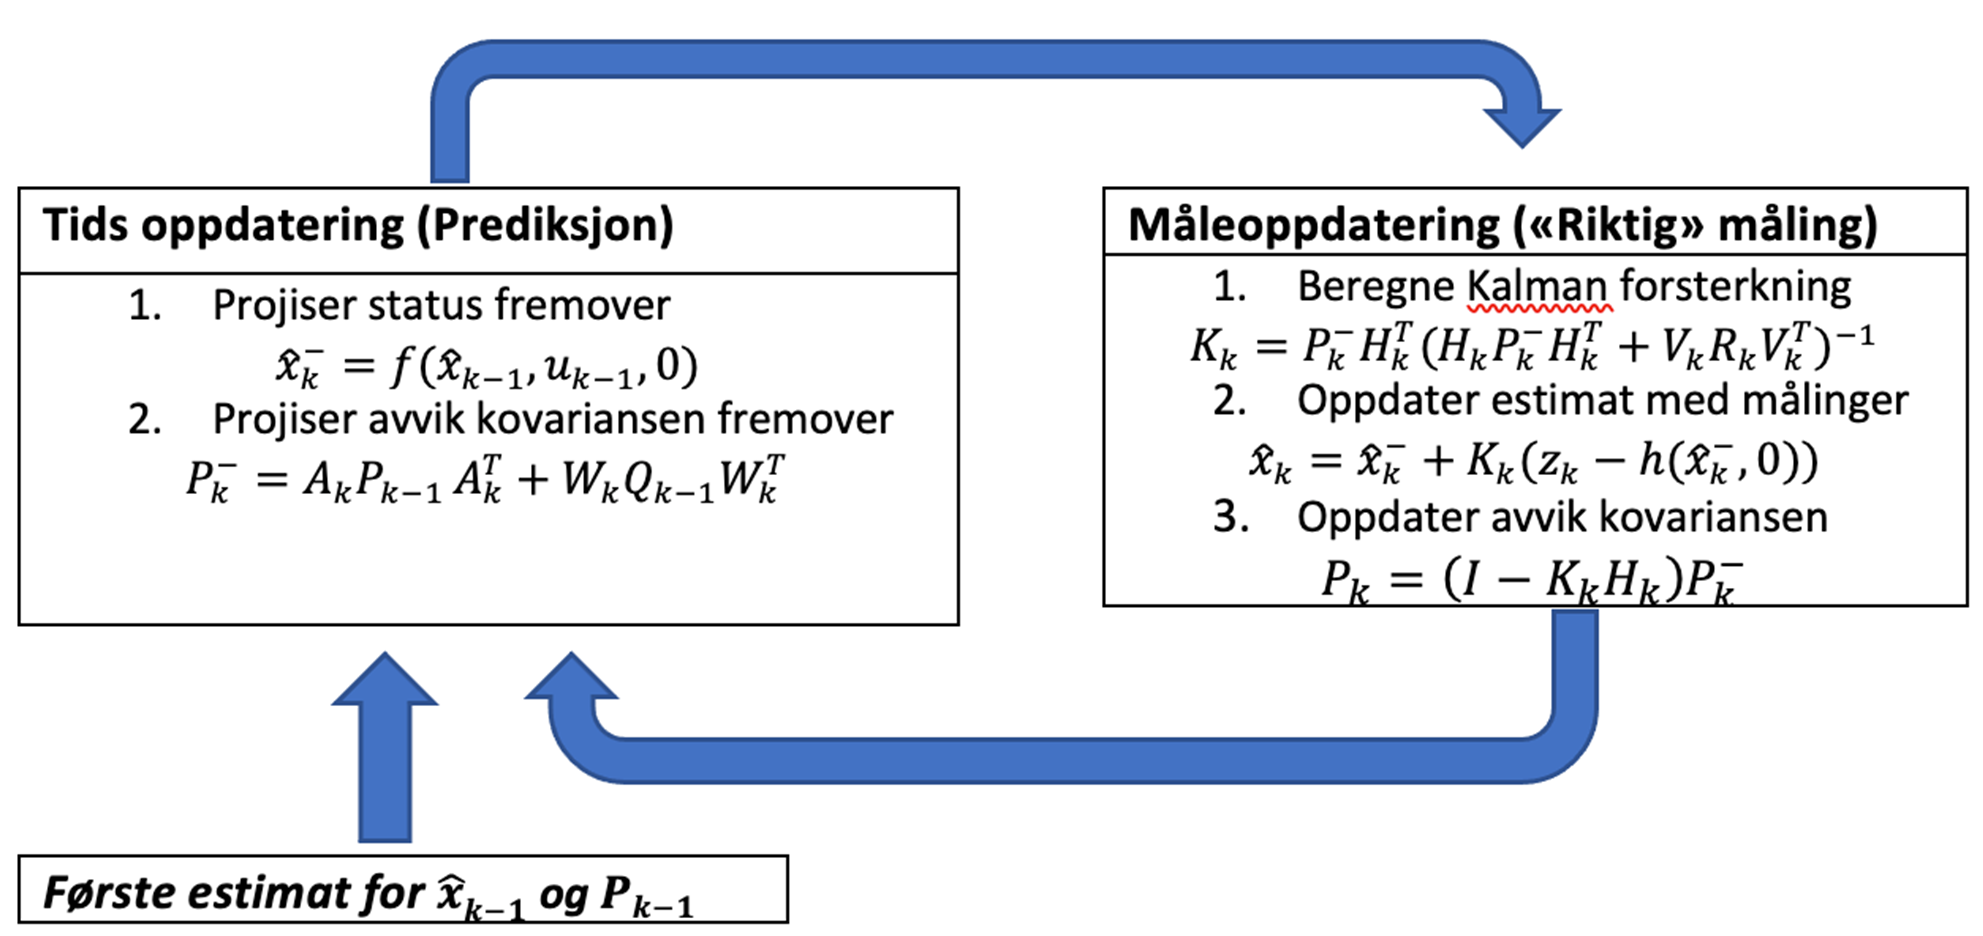
\includegraphics[width=1\columnwidth]{figures/ekf}
    \caption{EKF algoritme.}
    \label{fig:ekf}
\end{figure}

Figur \ref{fig:ekf} viser hvordan EKF oppdateres. EKF prediktere neste status på systemet fra forrige estimat og 
deretter korrigere dette estimatet med målinger i nåtid fra sensorer. For en drone vil sensorer fra IMU og kompass 
gi rotasjon og akselerasjon. GNSS eller andre posisjonssystem og barometer vil kunne gi posisjonen og høyden til dronen. 
EKF samler dataen fra sensorene og gir estimat på posisjon, og rotasjon, fart og akselerasjon. 
Dette estimatet kan vider bli brukt til å regulere dronen sitt pådrag for å styre dronen, 
dette kommer rapporten mer inn på i PID-regulering avsnittet. \parencite{ArdupilotDevTeam}
